\documentclass{article}
\usepackage{amsmath}
\usepackage{courier}
\usepackage{enumerate}
\usepackage{fullpage}
\usepackage{graphicx}
\renewcommand{\vec}[1]{\boldsymbol{#1}}
\newcommand{\pd}[2]{\frac{\partial#1}{\partial#2}}
\newcommand{\var}{\mathop{\mathrm{Var}}}

\title{Statistics 221 Final Project: C++ team}
\author{Adam Petcher, Brandon Sim, Andrew Liu, Jason Sclar, Rohit Ramani}
\begin{document}
\maketitle

\section{Compare MLE to SGD}
MLE methods such Newton-Raphson compute the gradient of the log-likelihood, $\nabla\ell$ for all observations in one step. While this works well for small samples, it is too computationally expensive to be done with especially large amounts of data. Sakrison's method relies on the assumption that the expectation of the gradient for a single observation is proportional to the gradient for all observations. By the law of large numbers, repeatedly updating using the gradient for single observations will converge to expectations. This makes it possible to do the update step for a single observation at a time and compute the MLE.

The implicit updates use the update step, $\vec{\theta}_{t+1} = \vec{\theta}_t + a_t\nabla\ell(\vec{\theta}_{t+1}; y_t, \vec{x}_t)$ instead of $\vec{\theta}_{t+1} = \vec{\theta}_t + a_t\nabla\ell(\vec{\theta}_{t}; y_t, \vec{x}_t)$. However the expectation of the gradient is the same for all observations. Therefore $\nabla\ell(\vec{\theta}_{t+1}; y_t, \vec{x}_t) = \nabla\ell(\vec{\theta}_{t}; y_t, \vec{x}_t)$. Since the implicit method has the same expectation as Sakrison's method, it must also compute the MLE.


\section{GLM Proofs}

\begin{enumerate}[(a)]
\item Show $E(y_t|\vec{x}_t) = h(\vec{x}_t^T\vec{\theta}^*) = b'(\eta_t)$ \\
We start with the moment generating function, which we solve for using LOTUS
\begin{align*}
M_Y(t) &= E[e^{tY}]\\
&= \int_Y \exp(ty_k)f(y_k|\eta_k)dy_k\\
&= \int_Y \exp(ty_k)\exp\bigg(\frac{\eta_ty_t - b(\eta_t)}{\phi}\bigg)\cdot c(y_t, \phi)dy_k\\
&= \int_Y c(y_t, \phi)\exp\bigg(ty_k + \frac{\eta_ty_t}{\phi} - \frac{b(\eta_t)}{\phi}\bigg) dy_k\\
&= \int_Y c(y_t, \phi)\exp\bigg(\bigg(\frac{\eta_ty_t + \phi t}{\phi}\bigg)y_k - \frac{b(\eta_t)}{\phi}\bigg) dy_k\\
&= \int_Y c(y_t, \phi)\exp\bigg(\bigg(\frac{\eta_ty_t + \phi t}{\phi}\bigg)y_k - \frac{b(\eta_k + \phi t)}{\phi} + \frac{b(\eta_k + \phi t)}{\phi} - \frac{b(\eta_t)}{\phi}\bigg) dy_k\\
&= \int_Y \exp\bigg(\frac{b(\eta_k + \phi t) - b(\eta_t)}{\phi}\bigg)c(y_t, \phi)\exp\bigg(\frac{(\eta_ty_t + \phi t) y_k - b(\eta_k + \phi t)}{\phi}\bigg) dy_k\\
&= \exp\bigg(\frac{b(\eta_k + \phi t) - b(\eta_t)}{\phi}\bigg)\int_Y c(y_t, \phi)\exp\bigg(\frac{(\eta_ty_t + \phi t) y_k - b(\eta_k + \phi t)}{\phi}\bigg) dy_k\\
\end{align*}
The remaining integral is the conditional pdf of $y|\eta_k + \phi t$ and integrates to 1, which leaves the remaining MGF for $Y$
$$M_Y(t) = \exp\bigg(\frac{b(\eta_k + \phi t) - b(\eta_t)}{\phi}\bigg) $$
We then use the MGF to find $E(y_t|\vec{x}_t)$. We start by finding $M'_Y(t)$
\begin{align*}
M'_Y(t) &= \pd{}{t} \bigg[\exp\bigg(\frac{b(\eta_k + \phi t) - b(\eta_t)}{\phi}\bigg)\bigg]\\
&= \exp\bigg(\frac{b(\eta_k + \phi t) - b(\eta_t)}{\phi}\bigg)\cdot\frac{b'(\eta_k + \phi t)\phi}{\phi}\\
&= \exp\bigg(\frac{b(\eta_k + \phi t) - b(\eta_t)}{\phi}\bigg)\cdot b'(\eta_k + \phi t)\\
\end{align*}
We then evaluate at $t=0$ which is the first moment.
\begin{align*}
E(y_t|\vec{x}_t) &= M'_Y(0)\\
&= \exp\bigg(\frac{b(\eta_k + \phi\cdot 0) - b(\eta_t)}{\phi}\bigg)\cdot b'(\eta_k + \phi\cdot 0)\\
&= \exp\bigg(\frac{0}{\phi}\bigg)\cdot b'(\eta_k)\\
&= b'(\eta_k)\\
\end{align*}

\item Show $\var(y_t|\eta_t) = \phi\cdot h'(\eta_t)$\\
We find the variance using the moment generating function from part (a).
$$\var(y_k|\eta_k) = E(y^2_k|\eta_k) - [E(y_k|\eta_k)]^2$$
We can use the value of $E(y_k|\eta_k)$ from part (a). We then find the second moment $E(y^2_k|\eta_k)$ with our MGF.
\begin{align*}
M''_Y(t) =& \pd{}{t} \bigg[\exp\bigg(\frac{b(\eta_k + \phi t) - b(\eta_t)}{\phi}\bigg)\cdot b'(\eta_k + \phi t)\bigg]\\
=& \exp\bigg(\frac{b(\eta_k + \phi t) - b(\eta_t)}{\phi}\bigg)\cdot b'(\eta_k + \phi t)\cdot b'(\eta_k + \phi t) +\\
& b''(\eta_k + \phi t)\cdot\phi\cdot\exp\bigg(\frac{b(\eta_k + \phi t) - b(\eta_t)}{\phi}\bigg)\\
=& \exp\bigg(\frac{b(\eta_k + \phi t) - b(\eta_t)}{\phi}\bigg)\cdot \bigg[b'(\eta_k + \phi t)\bigg]^2 + b''(\eta_k + \phi t)\cdot\phi\cdot\exp\bigg(\frac{b(\eta_k + \phi t) - b(\eta_t)}{\phi}\bigg)\\
\end{align*}
Evaluating at 0 gives
\begin{align*}
 E(y^2_k|\eta_k) =& M''_Y(0)\\
=& \exp\bigg(\frac{b(\eta_k + \phi *0) - b(\eta_t)}{\phi}\bigg)\bigg[b'(\eta_k + \phi *0)\bigg]^2 + b''(\eta_k + \phi *0)\phi\exp\bigg(\frac{b(\eta_k + \phi *0) - b(\eta_t)}{\phi}\bigg)\\
=& \exp(\frac{0}{\phi})\bigg[b'(\eta_k)\bigg]^2 + \phi \cdot b''(\eta_k)\exp(\frac{0}{\phi})\\
=& \bigg[b'(\eta_k)\bigg]^2 + \phi \cdot b''(\eta_k)\\
\end{align*}
Putting the two parts together gives the solution
\begin{align*}
\var(y_t|\eta_t) &= E(y^2_k|\eta_k) -  [E(y_k|\eta_k)]^2\\
&= [b'(\eta_k)]^2 + \phi \cdot b''(\eta_k) -  [b'(\eta_k)]^2\\
&= \phi \cdot b''(\eta_k)\\
\end{align*}
From part (a) we know that $b'(\eta_t) = h(\eta)$ therefore $b''(\eta_t) = h'(\eta_t)$ which gives
$$\var(y_t|\eta_t) = \phi\cdot h'(\eta_t)$$

\item Show $\nabla\ell(\vec{\theta}; y_t, \vec{x}_t) = \frac{1}{\phi}(y_t - h(\vec{x}_t^T\theta))\vec{x}_t$\\
To find $\nabla\ell(\vec{\theta}; y_t, \vec{x}_t)$, we take the partial derivative with respect to $\vec{\theta}$. The likelihood is proportional to the pdf.
\begin{align*}
L(\vec{\theta}; y_t, \vec{x}_t) &\propto \exp\bigg(\frac{\eta_ty_t - b(\eta_t)}{\phi}\bigg)\cdot c(y_t, \phi)\\
\ell(\vec{\theta}; y_t, \vec{x}_t) &=  \frac{\eta_ty_t - b(\eta_t)}{\phi}\\
\nabla\ell(\vec{\theta}; y_t, \vec{x}_t) &= \pd{}{\vec{\theta}}\bigg[\ell(\vec{\theta}; y_t, \vec{x}_t)\bigg]\\
&= \pd{}{\vec{\theta}}\bigg[\frac{\eta_ty_t - b(\eta_t)}{\phi}\bigg]\\
&= \pd{}{\vec{\theta}}\bigg[\frac{\vec{x}_t^T\vec{\theta}y_t - b(\vec{x}_t^T\vec{\theta})}{\phi}\bigg]\\
&= \frac{1}{\phi}(\vec{x}_ty_t - \vec{x}_tb'(\vec{x}_t^T\vec{\theta}))\\
&= \frac{1}{\phi}(y_t - h(\vec{x}_t^T\vec{\theta}))\vec{x}_t\\
\end{align*}

\item Show $\mathcal{J}(\vec{\theta}) = -E(\nabla\nabla\ell(\vec{\theta}; y_t, \vec{x}_t)) = \frac{1}{\phi}E(h'(\vec{x}_t^T\vec{\theta})\vec{x}_t\vec{x}_t')$\\
To find the Fisher information, we take the negative expectation of the second partial derivative of the log-likelihood with respect to $\vec{\theta}$. We start with the the solution from part (c).
\begin{align*}
\mathcal{J}(\vec{\theta}) &= -E\bigg(\nabla\nabla\ell(\vec{\theta}; y_t, \vec{x}_t)\bigg)\\
&= -E\bigg(\pd{}{\vec{\theta}}\bigg[\frac{1}{\phi}(y_t - h(\vec{x}_t^T\vec{\theta}))\vec{x}_t\bigg]\bigg)\\
&= -E\bigg(-\frac{1}{\phi}\cdot h'(\vec{x}_t^T\vec{\theta})\vec{x}_t\vec{x}_t^T\bigg)\\
&= \frac{1}{\phi}\bigg(h'(\vec{x}_t^T\vec{\theta})\vec{x}_t\vec{x}_t^T\bigg)\\
\end{align*}

\end{enumerate}

\section{Implementation and Results}

\begin{enumerate}[(a)]
\item \textbf{Log-loss.} The log-loss function is given by:
\begin{equation}
L(y, \hat{y}) = \log(1+\exp(-y\hat{y}))
\end{equation}
The SGD update is given by:
\begin{equation}
\vec{\theta_{t+1}} = \vec{\theta_{t}} - \alpha_{t}\nabla Q(\vec{\theta_{t}}, y_t, \vec{x_t})
\end{equation}
where
\begin{equation}
Q(\vec{\theta_{t}}, y_t, \vec{x_t}) = \log\left(1+\exp(-y_t\cdot\vec{x_t^{T}}\vec{\theta_t})\right) + \frac{\lambda}{2}\|\vec{\theta_t}\|^2
\end{equation}
The gradient $\nabla Q(\vec{\theta_{t}}, y_t, \vec{x_t})$ can be calculated as follows:
\begin{align*}
\nabla Q(\vec{\theta_{t}}, y_t, \vec{x_t}) &= \left(\frac{1}{1+\exp(-y_t\cdot\vec{x_t^{T}}\vec{\theta_t})} \right)\left(\exp(-y_t\cdot\vec{x_t^{T}}\vec{\theta_t})\right)\left(-y_t\cdot\vec{x_t}\right) + \lambda\vec{\theta_t}\\
&= \frac{-y_t\exp(-y_t\cdot\vec{x_t^{T}}\vec{\theta_t})}{1+\exp(-y_t\cdot\vec{x_t^{T}}\vec{\theta_t})}\cdot\vec{x_t} + \lambda\vec{\theta_t}\\
\end{align*}
The implicit update can be derived in much the same way as above. We have the following:
\begin{align*}
&= \frac{-y_t}{\exp(y_t\cdot\vec{x_t^{T}}\vec{\theta_t})+1}\cdot\vec{x_t} + \lambda\vec{\theta_t}
\vec{\theta_{t+1}} &= \vec{\theta_t} - \alpha_t \nabla Q(\vec{\theta_{t+1}}, y_t, \vec{x_t})\\
&= \vec{\theta_t} - \alpha_t \left(\frac{-y_t}{\exp(y_t\cdot\vec{x_t^{T}}\vec{\theta_{t+1}})+1}\cdot\vec{x_t} + \lambda\vec{\theta_{t+1}} \right)
\end{align*}\\

\textbf{Hinge-loss.} The hinge loss function is given by:
\begin{equation}
L(y, \hat{y}) = \max(0, 1-y\hat{y})
\end{equation}
The SGD update is given by:
\begin{equation}
\vec{\theta_{t+1}} = \vec{\theta_{t}} - \alpha_{t}\nabla Q(\vec{\theta_{t}}, y_t, \vec{x_t})
\end{equation}

where

\begin{equation}
Q(\vec{\theta_{t}}, y_t, \vec{x_t}) = \max(0, 1-y_t\cdot\vec{x_t^{T}}\vec{\theta_t}) + \frac{\lambda}{2}\|\vec{\theta_t}\|^2
\end{equation}

The gradient $\nabla Q(\vec{\theta_{t}}, y_t, \vec{x_t})$ can be calculated as follows, where we consider two cases depending on the sign of $1-y_t\cdot\vec{x_t^{T}}\vec{\theta_t}$:

\begin{enumerate}[1.]
\item If $1-y_t\cdot\vec{x_t^{T}}\vec{\theta_t} < 0$, then $Q(\vec{\theta_{t}}, y_t, \vec{x_t}) = \frac{\lambda}{2}\|\vec{\theta_t}\|^2$. Then,

\begin{align*}
\nabla Q(\vec{\theta_{t}}, y_t, \vec{x_t}) &= \nabla\left(\frac{\lambda}{2}\|\vec{\theta_t}\|^2\right)\\
&= \lambda \vec{\theta_t}
\end{align*}

\item If $1-y_t\cdot\vec{x_t^{T}}\vec{\theta_t} \geq 0$, then $Q(\vec{\theta_{t}}, y_t, \vec{x_t}) = 1-y_t\cdot\vec{x_t^{T}}\vec{\theta_t}+\frac{\lambda}{2}\|\vec{\theta_t}\|^2$. Then,

\begin{align*}
\nabla Q(\vec{\theta_{t}}, y_t, \vec{x_t}) &= \nabla\left(1-y_t\cdot\vec{x_t^{T}}\vec{\theta_t}+\frac{\lambda}{2}\|\vec{\theta_t}\|^2\right)\\
&= \nabla\left( -y_t\cdot\vec{x_t^{T}}\vec{\theta_t} \right) + \lambda \vec{\theta_t}\\
&= -y_t\cdot\vec{x_t} + \lambda\vec{\theta_t}
\end{align*}

where the last step is accomplished by noting that:
\begin{align*}
\nabla_{\theta}\left(\vec{x^{T}}\vec{\theta}\right) &= \nabla_{\theta}\left(\sum_{i=1}^{|\vec{x}|} x_i\theta_i\right)\\
&= \left( \pd{}{\theta_1}\left(\sum_{i=1}^{|\vec{x}|} x_i\theta_i\right), \pd{}{\theta_2}\left(\sum_{i=1}^{|\vec{x}|} x_i\theta_i\right), \ldots \right)\\
&= \left( x_1, x_2, \ldots \right)\\
&= \vec{x}
\end{align*}

\end{enumerate}

Putting these results together, we have that:
\begin{equation}
\vec{\theta_{t+1}} = \vec{\theta_t} - \alpha_t \left\{ 
	\begin{array}{lr}
		\lambda\vec{\theta_t} &  y_t\cdot\vec{x_t^{T}}\vec{\theta_t} > 1\\
		\lambda\vec{\theta_t} - y_t\vec{x_t} &  \textrm{otherwise}
	\end{array}
\right.
\end{equation}

We now derive the implicit update for the hinge loss, which is given by:
\begin{equation}
\vec{\theta_{t+1}} = \vec{\theta_{t}} - \alpha_{t}\nabla Q(\vec{\theta_{t+1}}, y_t, \vec{x_t})
\end{equation}

The calculations are very similar to the SGD derivation above, and for the two cases depending on the sign of $1-y_t\cdot\vec{x_t^{T}}\vec{\theta_{t+1}}$ are:

\begin{enumerate}[1.]
\item If $1-y_t\cdot\vec{x_t^{T}}\vec{\theta_{t+1}} < 0$, then
\begin{equation*}
\nabla Q(\vec{\theta_{t+1}}, y_t, \vec{x_t}) = \lambda\vec{\theta_{t+1}}
\end{equation*}

Then, substituting this result into the implicit update equation above, we can solve to find:
\begin{equation}
\vec{\theta_{t+1}} = \frac{1}{1+\lambda\alpha_t}\vec{\theta_t}
\end{equation}

\item If $1-y_t\cdot\vec{x_t^{T}}\vec{\theta_{t+1}} \geq 0$, then 
\begin{equation*}
\nabla Q(\vec{\theta_{t+1}}, y_t, \vec{x_t}) = -y_t\cdot\vec{x_t} + \lambda\vec{\theta_{t+1}}
\end{equation*}
\end{enumerate}

Then, substituting this result into the implicit update equation above, we can solve to find:
\begin{equation}
\vec{\theta_{t+1}} = \frac{1}{1+\lambda\alpha_t}\left(\vec{\theta_t} + \alpha_t y_t\cdot\vec{x_t}\right)
\end{equation}

Note that during implementation, we should be careful to make sure that we check the sign of $1-y_t\cdot\vec{x_t^{T}}\vec{\theta_{t+1}}$ after the update, as the derivation of the implicit updates forced an assumption of the sign to begin with. If the assumption was wrong, then the other update function should be used.\\

\textbf{Squared-loss.}
The squared-loss function is given by:
\begin{equation}
L(y, \hat{y}) = (y-\hat{y})^2
\end{equation}

The SGD update is given by:
\begin{equation}
\vec{\theta_{t+1}} = \vec{\theta_{t}} - \alpha_{t}\nabla Q(\vec{\theta_{t}}, y_t, \vec{x_t})
\end{equation}

where

\begin{equation}
Q(\vec{\theta_{t}}, y_t, \vec{x_t}) = \left(y_t - \vec{x_t^T}\vec{\theta_t}\right)^2 + \frac{\lambda}{2}\|\vec{\theta_t}\|^2
\end{equation}

The gradient $\nabla Q(\vec{\theta_{t}}, y_t, \vec{x_t})$ can be calculated as follows:

\begin{align*}
\nabla Q(\vec{\theta_{t}}, y_t, \vec{x_t}) &= 2\left(y_t - \vec{x_t^T}\vec{\theta_t}\right)\left(-\vec{x_t}\right) + \lambda\vec{\theta_t}\\
&= -2(y_t-\vec{x_t^T}\vec{\theta_t})\vec{x_t} + \lambda\vec{\theta_t}\\
\end{align*}

So, the SGD update for the log-loss function is:
\begin{equation}
\vec{\theta_{t+1}} = \vec{\theta_{t}} +2 \alpha_{t}\left( y_t-\vec{x_t^T}\vec{\theta_t} \right )\vec{x_t} - \alpha_t\lambda\vec{\theta_t}
\end{equation}

The implicit update can be derived in much the same way as above. We have the following:

\begin{align*}
\vec{\theta_{t+1}} &= \vec{\theta_t} - \alpha_t \nabla Q(\vec{\theta_{t+1}}, y_t, \vec{x_t})\\
\vec{\theta_{t+1}} &= \vec{\theta_{t}} +2 \alpha_{t}\left( y_t-\vec{x_t^T}\vec{\theta_{t+1}} \right )\vec{x_t} - \alpha_t\lambda\vec{\theta_{t+1}}\\
(1+\alpha_t\lambda)\vec{\theta_{t+1}} &= \vec{\theta_{t}} +2 \alpha_{t}\left( y_t-\vec{x_t^T}\vec{\theta_{t+1}} \right )\vec{x_t}\\
(1+\alpha_t\lambda)\vec{\theta_{t+1}} &= \vec{\theta_{t}} + 2\alpha_t y_t \vec{x_t} - 2\alpha_t\vec{x_t^T}\vec{\theta_{t+1}}\vec{x_t}\\
\left[(1+\alpha_t\lambda)I + 2\alpha_t\vec{x_t^T}\vec{x_t}I\right]\vec{\theta_{t+1}} &= \vec{\theta_t} + 2\alpha_t y_t\vec{x_t}\\
\vec{\theta_{t+1}} &= \left[(1+\alpha_t\lambda)I + 2\alpha_t\vec{x_t^T}\vec{x_t}I\right]^{-1}\left(\vec{\theta_t} + 2\alpha_t y_t \vec{x_t}\right)
\end{align*}

\item We downloaded and compiled Bottou's SGD package.
\item See \texttt{svmimplicit.cpp}.
\item Here we report the results from running the SGD experiment. We compare performance of baseline SGD, ASGD, and our implicit SGD for each of the log loss and hinge loss functions and each of the RCV1 and alpha datasets across three metrics: training time, test (misclassification) error, and cost, measured as  $$C = L + 0.5 \lambda ||\Theta||^2$$ where $L$ denotes the average loss over all test runs and $\Theta$ the parameter vector. (We leave out LibLinear because we could not format the data correctly in time.) We ran all the experiments on Andrew's personal computer using one core, and the longest run in terms of computation time that we tried was approximately 20 seconds. Each run was done individually from the command line (instead of packaging all runs into one script) for easier debugging and due to the small number of runs necessary.

Unless otherwise stated, SGD algorithms use their default regularization parameters (close to $\lambda = 10^{-5}$) and learning rate $\eta_t = \frac{\eta_0}{1+ \lambda\eta_0 t}$ as specified in the Bottou SVM README, with $\eta_0$ picked by the Bottou package unless otherwise specified. We chose these regularization parameters because they optimized the performance of each run.

\begin{enumerate}[1.]
\item RCV1 Benchmark, hinge-loss.
\begin{center}
\begin{tabular}{ c | c | c | c }
  algorithm & training time (s) & test error (\%) & cost \\ \hline                       
  SGD & 0.87 &  6.005 & 0.244\\
  ASGD & 0.86 & 6.018 & 0.244\\
  Implicit & 0.71 & 5.184 & 0.144\\
\end{tabular}
\end{center}

\item RCV1 Benchmark, log-loss.
\begin{center}
\begin{tabular}{ c | c | c | c }
  algorithm & training time (s) & test error (\%) & cost \\ \hline                       
  SGD & 3.47 &  5.175 & 0.153\\
  ASGD & 4.03 & 5.145 & 0.154\\
  Implicit ($\eta_0=10$, not 4) & 1.92 & 5.262 & 0.537\\
\end{tabular}
\end{center}
For implicit SGD, I use learning rate $\eta_t = \frac{\eta_0}{1+ \lambda\eta_0 t/2}$.

\item Alpha dataset, hinge-loss.
\begin{center}
\begin{tabular}{ c | c | c | c }
  algorithm & training time (s) & test error (\%) & cost \\ \hline                       
  SGD & 3.37 & 22.7 & 0.548\\
  ASGD & 2.27 & 21.83 & 0.532\\
  Implicit ($\eta_0=10$, not 0.25) & 2.29 & 22.18 & 0.565\\
\end{tabular}
\end{center}
Implicit SGD here was improved by using default $\lambda = 10^{-5}$ (whereas SGD and ASGD used $\lambda = 10^{-6}$).

\item Alpha dataset, log-loss.
\begin{center}
\begin{tabular}{ c | c | c | c }
  algorithm & training time (s) & test error (\%) & cost \\ \hline                       
  SGD & 9.31 &  22.11 & 0.477\\
  ASGD & 3.5 & 21.9 & 0.474\\
  Implicit ($\eta_0=10$, not 0.25) & 3.7 & 21.9 & 0.542\\
\end{tabular}
\end{center}
\end{enumerate}
\end{enumerate}

We also wanted to test the robustness of each method to misspecification of parameters such as regularization rate and learning rate. Looking at our results, implicit SGD is only noticeably performing better (considering training time and test error) in hinge-loss on the RCV1 dataset, so we considered each algorithm's performance while varying its regularization rate. By taking the test error at the end of 1 second of training, we find that implicit SGD is slightly more robust to changes in regularization rate than the other two:

\begin{center}
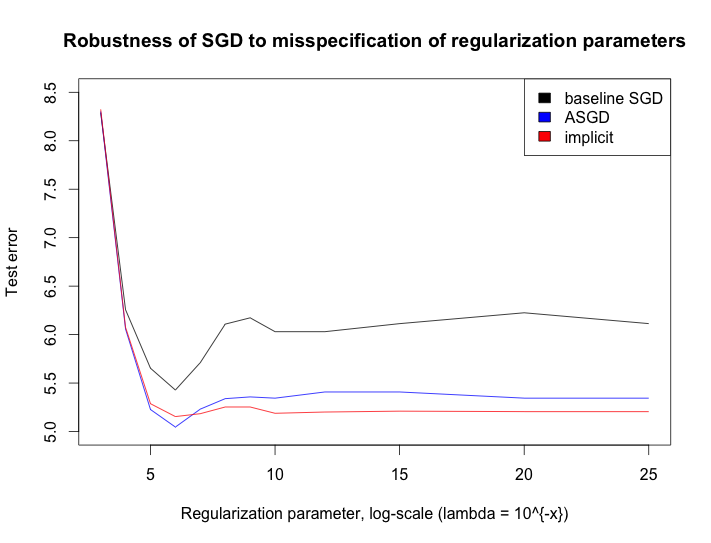
\includegraphics[width=140mm]{regularization_robustness.png}\\
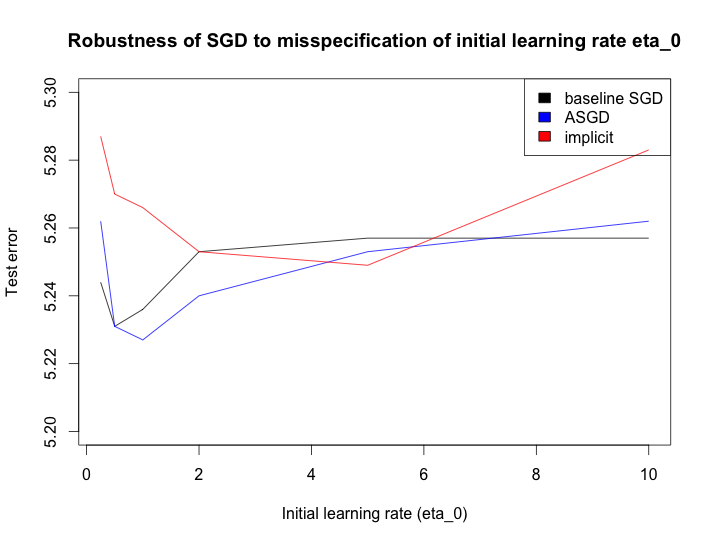
\includegraphics[width=140mm]{eta0_robustness.png}
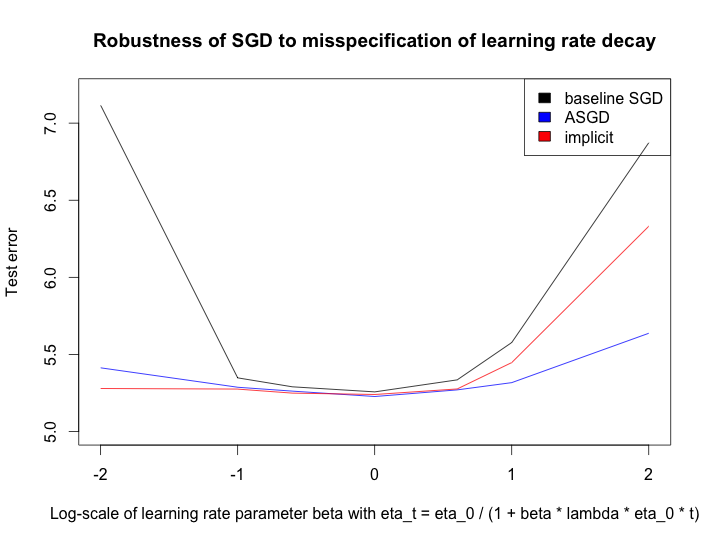
\includegraphics[width=140mm]{etat_robustness.png}
\end{center}

\section{Discussion}

Our first main result is that implicit SGD only outperformed baseline SGD and ASGD in both training time and test error in the hinge-loss case for the RCV1 dataset while doing as well or worse than ASGD in the other cases (and always better than baseline SGD). In hinge-loss for RCV1, implicit SGD converged slightly more quickly and with less error, and in log-loss, it converged more quickly than the other implementations but with slightly more error. In alpha, it converged at approximately the same rate as ASGD (and faster than baseline SGD) and had error on par with ASGD, and better than baseline SGD.

We hypothesized that our implicit SGD implementation would (a) have lower error than other implementations, fixing convergence time, and (b) have lower convergence time, fixing error. That this did not happen is likely not due to incorrect derivation equations but could follow from bugs in our implementation, since we checked our implicit SGD update equations with Panos. However, our implementations' performance is quite close to the SGD and ASGD from the Bottou package, which suggests that the update equations were coded correctly. A more likely source of this underperformance is the tradeoff between making our code faster and computing things exactly; for instance, the \texttt{FVector combine} function used for adding was more exact but slower. Another possible source of underperformance was our inability to account for nonzero bias in our classifier, which required us to set the bias for all our classifiers to be zero (including baseline SGD and ASGD). This restriction may have affected implicit SGD disproportionately.

Our second main result is that implicit SGD is more robust than both other SGDs to misspecifications in regularization coefficient, and more robust than baseline SGD in misspecifications in learning rates. First, analyzing the graph of regularization parameter versus test error, we see that implicit SGD achieves a dramatically lower test error than baseline SGD for values of $\lambda = 10^{-i}$ for $i \ge 4$ (which happens to be close to Bottou's recommended regularization coefficient $\lambda = 10^{-5}$) and a slightly lower test error than ASGD. Next, we analyzed the sensitivity of each implementation to initial learning rates $\eta_0$, finding no significant differences between each implementation's robustness while varying $\eta_0$ (all test errors were still confined to $(5.22,5.29)$ after taking the implementation test errors by 1 second of training time). However, we did find that our implicit SGD was more robust than baseline SGD to different rates of decay $\beta$ in the learning rate equation $$\eta_t = \frac{\eta_0}{1 + \beta \lambda \eta_0 t}$$ but ASGD is even more robust than our implicit SGD. This might be due to implicit SGD needing higher learning rates overall, so that the ranges of values on which implicit SGD versus ASGD are more robust differ.

\section{Contributions}
On the implementation side, Adam did a majority of the work, being the first to download Bottou's SGD package and get it working (1.4b), and implementing each of the loss functions with implicit update (1.4c), as well as working with Brandon to figure out some of the math associated with those updates. He also debugged the \texttt{svmimplicit.cpp} code and did a little tuning of the parameters.

On the analysis side, Brandon derived the SGD and implicit updates for the three loss functions (1.4a). Jason gave the intuition for Sakrison's method and the implicit method computing the MLE (1.1), and performed the derivations of the desired properties of GLMs (1.2).

Finishing off the implementation, Andrew ran Adam's implicit SGD, along with baseline SGD and AGSD, on RCV1 and alpha datasets, collecting training time, test error, and cost data (1.4d, e). He tried but failed to get LibLinear working. He also did a little work to compile each team member's tex into this writeup and wrote the results and discussion sections (including the plots and data tables).

Adam and Brandon made large contributions in terms of keeping the team going forward, communicating their progress to the group and ensuring the group stayed knowledgeable, and starting on their work early so that the rest of the team had an easier time finishing off the missing pieces at the end.

\end{document}